%!TEX root = ../larxxia.tex

\section{Vectors have magnitude and direction}
\label{sec:vhmd}
\secttoc
\index{magnitude|(}

\begin{quoted}{(Hamlet I.5:159--167)}
There are more things in heaven and earth, Horatio, than are dreamt of in your philosophy.
\end{quoted}

In the eighteenth century, astronomers needed to describe both the position and velocity of the \idx{planets}. 
Such a description required quantities which have both a magnitude and a direction.
Step outside, a wind blowing at~\(8\)\,m/s (metres per second) from the south-west has both a magnitude and direction.
Quantities that have the properties of both a magnitude and a 
direction are called \bfidx{vector}s (from the Latin for \emph{carrier}).

\begin{example}[displacement vector] \label{eg:disvec}
An important class of vectors are the so-called \bfidx{displacement vector}s.
Given two points in space, say~\(A\) and~\(B\), the displacement vector~\(\ovect{AB}\) is the directed line segment from the point~\(A\) to the point~\(B\)---as illustrated by the two displacement vectors \(\ovect{AB}\) and~\(\ovect{CD}\) in the margin.
\newcommand{\tmp}[6]{
  \addplot[blue,thick,quiver={u=#5-#2,v=#6-#3},-stealth] coordinates {(#2,#3)};
  \node[below] at (axis cs:#2,#3) {$#1$};
  \node[below] at (axis cs:#5,#6) {$#4$};}
\newcommand{\temp}[1]{\begin{tikzpicture} 
\begin{axis}[footnotesize,font=\footnotesize
  ,axis equal,  xlabel={$x_1$}, ylabel={$x_2$},
  {\ifnum0=#1 axis lines=none\else axis lines=middle,grid\fi}
  ,xmin=-1.5,xmax=4.5,ymin=-1.7,ymax=3.5
  ] 
  \tmp A12B43
  \tmp C2{-1}D{-1}3
  \ifnum0=#1\else\node[below] at (axis cs:0,0) {\quad$O$};\fi
\end{axis}
\end{tikzpicture}}
\marginpar{\temp0}
For example, if your home is at position~\(A\) and your school at position~\(B\), then travelling from home to school is to move by the amount of the displacement vector~\(\ovect{AB}\).

To be able to manipulate vectors we describe them with numbers.
For such numbers to have meaning they must be set in the context of a \idx{coordinate system}.
So choose an origin for the coordinate system, usually denoted~\(O\), and draw \idx{coordinate axes} in the plane (or space), as illustrated for the above two \idx{displacement vector}s.
Here the displacement vector~\(\ovect{AB}\) goes three units to the right and one unit up, so we denote it by the ordered pair of numbers~\(\ovect{AB}=(3,1)\).
\marginpar{\temp1}
Whereas the displacement vector~\(\ovect{CD}\) goes three units to the left and four units up, so we denote it by the ordered pair of numbers~\(\ovect{CD}=(-3,4)\).
Our choice of the origin~\(O\) does not affect the number representation of these vectors.
\end{example}


\needspace{6\baselineskip}
\begin{example}[position vector] \label{eg:posvec}
The next important class of vectors are the \bfidx{position vector}s.
Given some chosen fixed origin in space, then \(\ovect{OA}\)~is the \idx{position vector} of the point~\(A\).
\newcommand{\tmp}[3]{
  \addplot[blue,thick,quiver={u=#2,v=#3},-stealth] coordinates {(0,0)};
  \node[below] at (axis cs:#2,#3) {$#1$};}
\newcommand{\temp}[1]{\begin{tikzpicture} 
\begin{axis}[footnotesize,font=\footnotesize
  ,axis equal, xlabel={$x_1$}, ylabel={$x_2$},
  {\ifnum0=#1 axis lines=none\else axis lines=middle,grid\fi}
  ,xmin=-1.5,xmax=4.5,ymin=-1.7,ymax=3.5
  ] 
  \tmp A12\tmp B43
  \tmp C2{-1}\tmp D{-1}3
  \node[below] at (axis cs:0,0) {\quad$O$};
\end{axis}
\end{tikzpicture}}%
\marginpar{\temp{0}}%
The marginal picture illustrates the \idx{position vector}s of four points in the plane, given a chosen origin~\(O\).

Again, to be able to manipulate such vectors we describe them with numbers, and such numbers have meaning via a \idx{coordinate system}.
\marginpar{\temp{1}}
So draw \idx{coordinate axes} in the plane (or space), as illustrated for the above four \idx{position vector}s.
Here the \idx{position vector}~\(\ovect{OA}\) goes one unit to the right and two units up so we denote it by \(\ovect{OA}=(1,2)\).
Similarly, the position vectors \(\ovect{OB}=(4,3)\),  \(\ovect{OC}=(2,-1)\), and  \(\ovect{OD}=(-1,3)\).
Recognize that the ordered pairs of numbers in the position vectors are exactly the \idx{coordinates} of each of the specified end-points. 
\end{example}


\begin{example}[\idx{velocity vector}] 
Consider an airplane in level flight at \(900\)\,km/hr (kilometres per hour) to the east-north-east.
\newcommand{\tmp}[3]{
  \addplot[blue,thick,quiver={u=#2,v=#3},-stealth] coordinates {(0,0)};
  \node[above] at (axis cs:#2,#3) {#1};}
\newcommand{\temp}[1]{\begin{tikzpicture} 
\begin{axis}[tiny,font=\footnotesize
  ,axis equal, xlabel={East}, ylabel={North}
  ,axis lines=middle,
  {\ifcase#1 xtick={-9999},ytick={-9999} \or grid\fi}
  ,ymin=-1,xmin=-20,xmax=980,ymax=380
  ] 
  \tmp {\mbox{airplane\quad}}{831.5}{344.4}
  \node[below] at (axis cs:0,0) {\quad$O$};
  \ifcase#1\or
  \tmp {}{831.5}{0}
  \tmp {}{0}{344.4}
  \fi
\end{axis}
\end{tikzpicture}}%
\marginpar{\temp0}%
Choosing coordinate axes oriented to the East and the North, the direction of the airplane is at an angle~\(22.5^\circ\) from the East, as illustrated in the margin.
Trigonometry then tells us that the Eastward part of the speed of the airplane is \(900\cos(22.5^\circ)=831.5\)\,km/hr, whereas the Northward part of the speed is \(900\sin(22.5^\circ)=344.4\)\,km/hr (as indicated in the margin).
\marginpar{\temp1}%
Further, the airplane is in level flight, not going up or down, so in the third direction of space (vertically) its speed component is zero.
Putting these together forms the velocity vector \((831.5,344.4,0)\) in~km/hr in space.

Another airplane takes off from an airport at~\(360\)\,km/hr to the northwest and climbs at~\(2\)\,m/s.
The direction northwest is~\(45^\circ\) to the East-West lines and \(45^\circ\) to the North-South lines.  
Trigonometry then tells us that the Westward speed of the airplane is \(360\cos(45^\circ)=360\cos(\tfrac\pi4)=254.6\)\,km/hr, whereas the Northward speed is \(360\sin(45^\circ)=360\sin(\tfrac\pi4)=254.6\)\,km/hr as illustrated in the margin.
\marginpar{\begin{tikzpicture} 
\begin{axis}[footnotesize,font=\footnotesize
  ,axis equal, xlabel={East}, ylabel={North}
  ,axis lines=middle, grid
  ,ymin=-60,xmin=-299,xmax=99,ymax=349
  ] 
  \tmp {airplane}{-254.6}{254.6}
  \node[below] at (axis cs:0,0) {\quad$O$};
\end{axis}
\end{tikzpicture}}%
But West is the opposite direction to East, so if the coordinate system treats East as positive, then West must be negative.
Consequently, together with the climb in the vertical, the velocity vector is \((-254.6\)\,km/hr,\(254.6\)\,km/hr,\(2\,\)m/s\()\).
But it is best to avoid mixing units within a vector, so here convert all speeds to~m/s: here \(360\)\,km/hr upon dividing by~\(3600\)\,secs/hr and multiplying by \(1000\)\,m/km gives \(360\)\,km/hr\({}=100\)\,m/s.
Then the North and West speeds are both \(100\cos(\tfrac\pi4)=70.71\)\,m/s.
Consequently, the \idx{velocity vector} of the climbing airplane should be described as \((-70.71,70.71,2)\) in~m/s.
\end{example}


In applications, as these examples illustrate, the `physical' vector exists before the \idx{coordinate system}.
It is only when we choose a specific coordinate system that a `physical' vector gets expressed by numbers.
%When enmeshed deep in the difficulties of learning the marvellous properties of vectors and matrices it is all to easy to forget this important aspect.
Throughout, unless otherwise specified, this book assumes that vectors are expressed in what is called a \bfidx{standard coordinate system}.
\begin{itemize}
\item In the two dimensions of the plane the \idx{standard coordinate system} has two \idx{coordinate axes}, 
\marginpar{\begin{tikzpicture} 
\begin{axis}[footnotesize,font=\footnotesize
  ,axis equal, axis lines=middle, grid
  , xlabel={$x_1$}, ylabel={$x_2$}
  ,xmin=-1.5,xmax=4.9,ymin=-1.5,ymax=3.5
  ] 
  \node[below] at (axis cs:0,0) {\quad$O$};
\end{axis}
\end{tikzpicture}}%
one horizontal and one vertical at right-angles to each other, often labelled~\(x_1\) and~\(x_2\) respectively (as illustrated in the margin), although labels~\(x\) and~\(y\) are also common.%

\item In the three dimensions of space the \idx{standard coordinate system} has three \idx{coordinate axes}, 
\marginpar{\begin{tikzpicture} 
\begin{axis}[footnotesize,font=\footnotesize,view={55}{30}
  ,axis equal, axis lines=box, grid
  ,xlabel={$x_1$}, ylabel={$x_2$}, zlabel={$x_3$},label shift={-1.5ex}
  ] 
  \node[below] at (axis cs:0,0,0) {$O$};
  \addplot3[black,quiver={u=4,v=0,w=0},-stealth] coordinates {(-1,0,0)};
  \node[below] at (axis cs:3,0,0) {$x_1$};
  \addplot3[black,quiver={u=0,v=4,w=0},-stealth] coordinates {(0,-1,0)};
  \node[below] at (axis cs:0,3,0) {$x_2$};
  \addplot3[black,quiver={u=0,v=0,w=3.3},-stealth] coordinates {(0,0,-0.3)};
  \node[left] at (axis cs:0,0,3) {$x_3$};
\end{axis}
\end{tikzpicture}}%
two horizontal and one vertical all at right-angles to each other, often labelled~\(x_1\), \(x_2\) and~\(x_3\) respectively (as illustrated in the margin), although labels~\(x\), \(y\) and~\(z\) are also common.

\item Correspondingly, in so-called `\(n\)~dimensions' the \idx{standard coordinate system} has \(n\)~\idx{coordinate axes}, all at right-angles to each other, and often labelled \hlist xn, respectively.
\end{itemize}




\begin{definition} \label{def:vecs} 
Given a \idx{standard coordinate system} with \(n\)~\idx{coordinate axes}, all at \idx{right-angles} to each other, a \bfidx{vector} is an ordered \(n\)-tuple of real numbers \hlist xn\ equivalently written either as a row in \idx{parentheses} or as a column in \idx{brackets},
\begin{equation*}
(\hlist xn)=\begin{bmatrix} x_1\\x_2\\\vdots\\x_n \end{bmatrix}
\end{equation*}
(they mean the same, it is just more convenient to usually use a row in parentheses in text, and a column in brackets in displayed mathematics).
The real numbers \hlist xn\ are called the \bfidx{components} of the vector, and the number of components is termed its \bfidx{size} (here~\(n\)).
The \idx{components} are determined such that letting~\(X\) be the point with \idx{coordinates} \((\hlist xn)\) then the \idx{position vector}~\(\ovect{OX}\) has the same magnitude and direction as the vector denoted \((\hlist xn)\).
\begin{aside}
% AJR's photo, taken in Wales
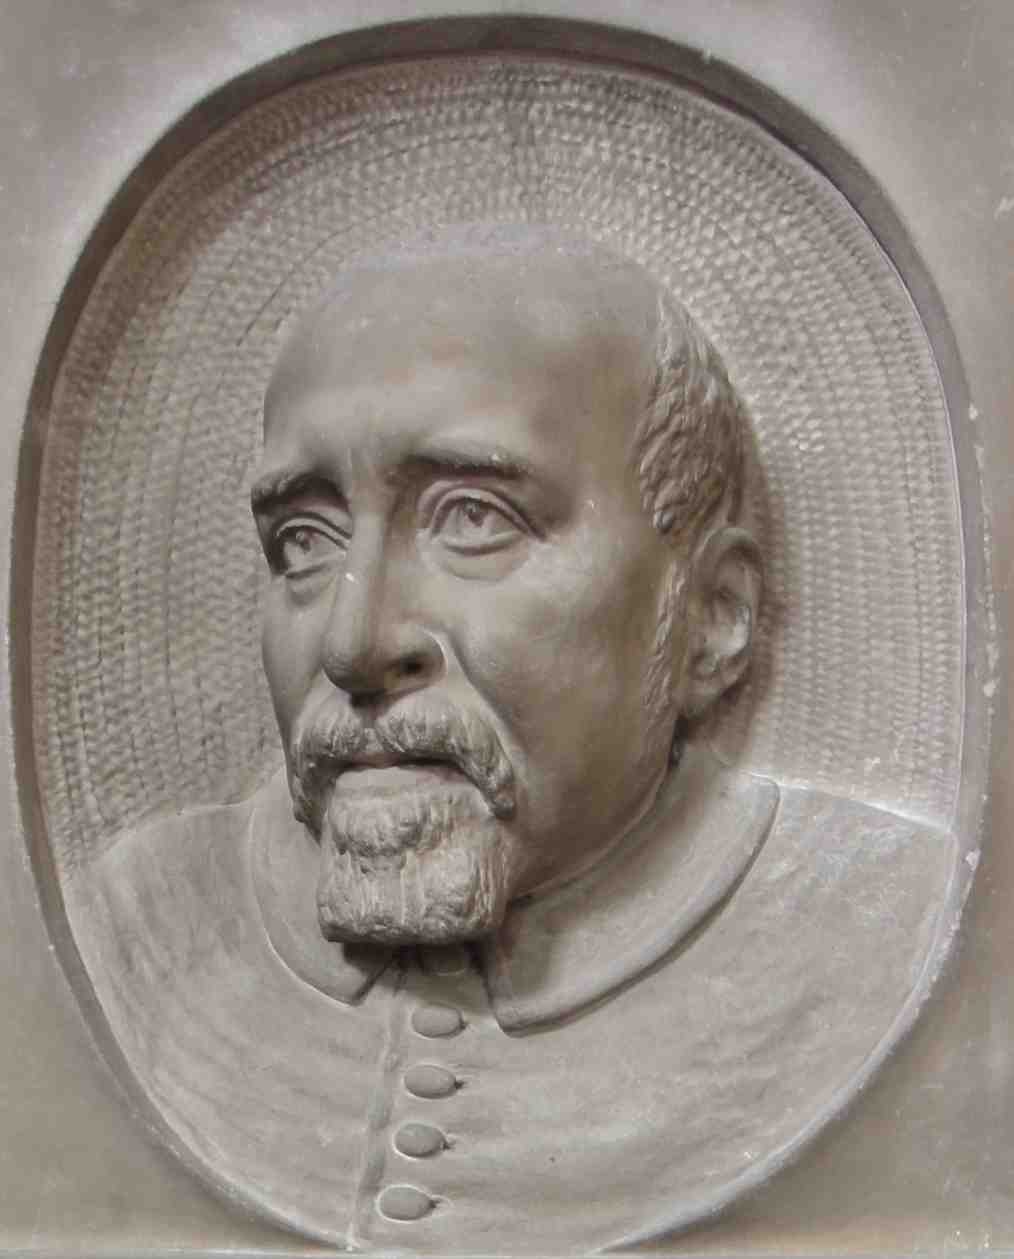
\includegraphics[width=\linewidth]{Vectors/RobertRecorde}
\index{Recorde, Robert}Robert Recorde invented the equal sign circa 1557 ``bicause noe~2 thynges can be moare equalle''.  
%He also invented the term ``sine'' and the method of extracting the square root by hand.
\end{aside}%
Two vectors of the same \idx{size} are \bfidx{equal},~\(=\), if all their corresponding \idx{components} are equal (vectors with different sizes are never equal).
\end{definition}

\cref{eg:disvec,eg:posvec} introduced some vectors and wrote them as a row in parentheses, such as \(\ovect{AB}=(3,1)\).
In this book exactly the same thing is meant by the columns in \idx{brackets}: for example,
\begin{eqnarray*}&&
\ovect{AB}=(3,1)=\begin{bmatrix} 3\\1 \end{bmatrix},\quad
\ovect{CD}=(-3,4)=\begin{bmatrix} -3\\4 \end{bmatrix},\quad
\\&&
\ovect{OC}=(2,-1)=\begin{bmatrix} 2\\-1 \end{bmatrix},\quad
(-70.71,70.71,2)=\begin{bmatrix} -70.71\\70.71\\2 \end{bmatrix}.
\end{eqnarray*}
However, as defined subsequently, a row of numbers within brackets is  quite different: for two examples, \((3,1)\neq\begin{bmatrix} 3&1 \end{bmatrix}\),  and \((831,344,0)\neq\begin{bmatrix} 831&344&0 \end{bmatrix}\).

The \emph{ordering} of the \idx{components} is very important.
\marginpar{\begin{tikzpicture} 
\newcommand{\tmp}[3]{
  \addplot[blue,thick,quiver={u=#2,v=#3},-stealth] coordinates {(0,0)};
  \node[below] at (axis cs:#2,#3) {$#1$};}
\begin{axis}[footnotesize,font=\footnotesize
  ,axis equal ,axis lines=middle, grid
  ,ymin=-1.9,xmin=-2,xmax=3.9,ymax=3.7
  ] 
  \tmp {\quad(3,1)}31 \tmp {\qquad(1,3)}13
  \tmp {\quad(2,-1)}2{-1} \tmp {(-1,2)\qquad}{-1}2
  \node[below] at (axis cs:0,0) {\quad$O$};
\end{axis}
\end{tikzpicture}}%
For example, as illustrated in the margin, the vector~\((3,1)\) is very different from the vector~\((1,3)\); similarly, the vector~\((2,-1)\) is very different from the vector~\((-1,2)\).
 


\begin{definition} \label{def:rRn}
The set of all vectors with \(n\)~\idx{components} is denoted~\(\RR^n\)\index{Rn@\(\RR^n\)}.
The vector with all components zero,  \((0,0,\ldots,0)\), is called the \bfidx{zero vector} and denoted by~\ov.
\end{definition}

\begin{example} 
\begin{itemize}
\item All the vectors we can draw and imagine in the two dimensional plane form~\(\RR^2\).  
Sometimes we write that \(\RR^2\)~is the plane because of this very close connection.

\item All the vectors we can draw and imagine in three dimensional space form~\(\RR^3\).  
Again, sometimes we write that \(\RR^3\)~is three dimensional space because of the close connection. 

\item The set~\(\RR^1\) is the set of all vectors with one component, and that one component is measured along one axis.  
Hence \(\RR^1\)~is effectively the same as the set of real numbers labelling that axis.
\blackqed
\end{itemize}
\end{example}


As just introduced for the zero vector~\ov, this book generally denotes vectors by a bold letter (except for \idx{displacement vector}s).
The other common notation you may see elsewhere is to denote vectors by a small over-arrow such as in the ``zero vector~\(\arrowvec0\)\,''.
Less commonly, some books and articles use an over- or under-tilde~(\(\sim\)) to denote vectors.
Be aware of this different notation in reading other books.



Question: why do we need vectors with \(n\)~components, in~\(\RR^n\), when the world around us is only three dimensional?
Answer: because vectors can encode much more than spatial structure as in the next example. 


\begin{example}[\idx{linguistic vector}s] \label{eg:deflsv}
Consider the following four sentences.
\begin{enumerate}
\item The dog sat on the mat.
\item The cat scratched the dog.
\item The cat and dog sat on the mat.
\item The dog scratched.
\end{enumerate}
These four sentences involve up to three objects, cat, dog and mat, and two actions, sat and scratched.  
Some characteristic of the sentences is captured simply by counting the number of times each of these three objects and two actions appear in each sentence, and then forming a vector from the counts.
Let's use vectors \(\wv=(N_{\text{cat}}, N_{\text{dog}}, N_{\text{mat}}, N_{\text{sat}}, N_{\text{scratched}})\) where the various~\(N\) are the counts of each word (\wv~for words). 
The previous statement implicitly specifies that we use five \idx{coordinate axes}, perhaps labelled ``cat'', ``dog'', ``mat'', ``sat'' and ``scratched'', and that distance along each axis represents the number of times the corresponding word is used.
These \idx{word vector}s are in~\(\RR^5\).
Then
\begin{enumerate}
\item ``The dog sat on the mat'' is summarized by the vector \(\wv=(0,1,1,1,0)\).
\item ``The cat scratched the dog'' is summarized by the vector \(\wv=(1,1,0,0,1)\).
\item ``The cat and dog sat on the mat'' is summarized by the vector \(\wv=(1,1,1,1,0)\).
\item ``The dog scratched'' is summarized by the vector \(\wv=(0,1,0,0,1)\).
\item An empty sentence is the \idx{zero vector} \(\wv=(0,0,0,0,0)\).
\item Together, the two sentences ``The dog sat on the mat.
 The cat scratched the dog.'' are summarized by the vector \(\wv=(1,2,1,1,1)\).
\end{enumerate}
Using such crude summary representations of some text, even of entire documents, empowers us to use powerful mathematical techniques to relate documents together, compare and contrast, express similarities, look for type clusters, and so on.
In application we would not just count words for objects (nouns) and actions (verbs), but also qualifications (adjectives and adverbs).\footnote{Look up Latent Semantic Analysis, such as at \url{https://en.wikipedia.org/wiki/Latent_semantic_analysis} [July 2019]}

People generally know and use thousands of words.
Consequently, in practice, such word vectors typically have thousands of components corresponding to coordinate axes of thousands of distinct words.
To cope with such vectors of many components, modern linear algebra has been developed to powerfully handle problems involving vectors with thousands, millions or even an `infinite number' of components.
\end{example}

\begin{table}
\hrule
\begin{minipage}{\linewidth}
\paragraph{King -- man + woman = queen}
\begin{quoted}{Technology Review, 2015}
Computational linguistics has dramatically changed the way researchers study and understand language. 
The ability to number-crunch huge amounts of words for the first time has led to entirely new ways of thinking about words and their relationship to one another.

This number-crunching shows exactly how often a word appears close to other words, an important factor in how they are used. 
So the word Olympics might appear close to words like running, jumping, and throwing but less often next to words like electron or stegosaurus.  
This set of relationships can be thought of as a multidimensional vector that describes how the word Olympics is used within a language, which itself can be thought of as a vector space.  

And therein lies this massive change. 
This new approach allows languages to be treated like vector spaces with precise mathematical properties. 
Now the study of language is becoming a problem of vector space mathematics.
\footnote{\url{http://www.technologyreview.com/view/541356} [Oct 2015]}
\end{quoted}
\end{minipage}
\hrule
\end{table}




\begin{activity}
Given \idx{word vector}s \(\wv=(N_{\text{cat}}\clb N_{\text{dog}}\clb N_{\text{mat}}\clb N_{\text{sat}}\clb N_{\text{scratched}})\) as in \cref{eg:deflsv},
which of the following has word vector \(\wv=(2,2,0,2,1)\)?
\actposs[1]
{``A dog sat.  A cat scratched the dog.  The cat sat.''}
{``The dog scratched the cat on the mat.''}
{``A dog and cat both sat on the mat which the dog had scratched.''}
{``Which cat sat by the dog on the mat, and then scratched the dog.''}
%\begin{enumerate}
%\item ``The dog scratched the cat on the mat.''
%\item\actans ``A dog sat.  A cat scratched the dog.  The cat sat.''
%\item ``A dog and cat both sat on the mat which the dog had scratched.''
%\item ``Which cat sat by the dog on the mat, and then scratched the dog.''
%\end{enumerate}
\end{activity}







\begin{definition}[Pythagoras] \label{def:veclen}
For every \idx{vector} \(\vv=(\hlist vn)\) in~\(\RR^n\),
define the \bfidx{length} (or \bfidx{magnitude}) of vector~\vv\  to be the real number~(\(\geq0\))
\index{$\vert\cdot\vert$|textbf} 
\begin{equation*}
|\vv|:=\sqrt{v_1^2+v_2^2+\cdots+v_n^2}\,.
\end{equation*}
A vector of length one is called a \bfidx{unit vector}.
(Many people and books denote the length of a vector with a pair of double lines, as in~\(\|\vv\|\).  Either notation is good.)
\end{definition}

\begin{example} 
Find the \idx{length}s of the following vectors.
\begin{Parts}
\item \(\eaii=(-3,4)\)
\begin{solution} 
\(|\eaii|=\sqrt{(-3)^2+4^2}=\sqrt{25}=5\). 
\end{solution}

\begin{reduce}
\item \(\eaii=(3,3)\)
\begin{solution} 
\(|\eaii|=\sqrt{3^2+3^2}=\sqrt{18}=3\sqrt2\). 
\end{solution}
\end{reduce}

\item \(\eaii=(1,-2,3)\)
\begin{solution} 
\(|\eaii|=\sqrt{1^2+(-2)^2+3^2}=\sqrt{14}\). 
\end{solution}

\begin{reduce}
\item \(\eaii=(1,-1,-1,1)\)
\begin{solution} 
\(|\eaii|=\sqrt{1^2+(-1)^2+(-1)^2+1^2}=\sqrt4=2\).
\end{solution}
\end{reduce}

\end{Parts}
\end{example}

\begin{example} 
Write down three different vectors, all three with the same number of components, that are (a)~of \idx{length}~\(5\), (b)~of length~\(3\), and (c)~of length~\(-2\).
\begin{solution} 
\begin{enumerate}
\item Humans knew of the \(3:4:5\) right-angled triangle thousands of years ago, so perhaps one answer could be \((3,4)\), \((-4,3)\) and~\((5,0)\).
\item One answer might be \((3,0,0)\), \((0,3,0)\) and~\((0,0,3)\). 
A more interesting answer might arise from knowing \(1^2+2^2+2^2=3^2\) leading to an answer of \((1,2,2)\), \((2,-1,2)\) and~\((-2,2,1)\).
\item Since the length of a vector is~\(\sqrt{\cdots}\) which is always positive or zero, the length cannot be negative, so there is no possible answer to this last request.
\end{enumerate}
 
\end{solution}
\end{example}




\begin{activity}
What is the \idx{length} of the vector \((2,-3,6)\)\,?
\actposs[4]{\(7\)}{\(\sqrt{11}\)}{\(5\)}{\(11\)}
\end{activity}




\begin{theorem} \label{thm:veclen0}
The \idx{zero vector} is the only vector of \idx{length} zero:
 \(|\vv|=0\) if and only if \(\vv=\ov\)\,.
\end{theorem}

\begin{proof} 
First establish the zero vector has length zero.
From \cref{def:veclen}, in~\(\RR^n\),
\begin{equation*}
|\ov|=\sqrt{0^2+0^2+\cdots+0^2}=\sqrt{0}=0\,.
\end{equation*}
Second establish that if a vector has length zero then it must be the zero vector.
Let vector \(\vv=(\hlist vn)\) in~\(\RR^n\) have zero length.
By squaring both sides of the \cref{def:veclen} for length we then know that
\begin{equation*}
\underbrace{v_1^2}_{\geq0}+\underbrace{v_2^2}_{\geq0}
+\cdots+\underbrace{v_n^2}_{\geq0}=0\,.
\end{equation*}
Being squares, all terms on the left are non-negative, so the only way they can all add to zero is if they are all zero.
That is, \(v_1=v_2=\cdots=v_n=0\)\,.
Hence, the vector~\vv\ must be the zero vector~\ov.
\end{proof}






\sectionExercises


\begin{exercise}  
For each case: on the plot draw the \idx{displacement vector}s \(\ovect{AB}\) and~\(\ovect{CD}\), and the \idx{position vector}s of the points~\(A\) and~\(D\).
\newcommand{\mytemp}{\begin{tikzpicture} 
\begin{axis}[footnotesize,font=\footnotesize
  ,axis equal, xlabel={$x_1$}, ylabel={$x_2$}
  ,axis lines=none  ] 
  \foreach \q in {A,B,C,D} {
    \pgfmathparse{rand*4}\let\h\pgfmathresult
    \pgfmathparse{rand*3}\let\v\pgfmathresult
    \edef\myytmp{\noexpand
    \addplot[blue,mark=*] coordinates {(\h,\v)} node[right] {$\q$};
    \noexpand \addplot[blue,no marks] coordinates {(0.5+\h,1.2*\v)};
    }\myytmp
    };
    \addplot[black,mark=*] coordinates {(0,0)} node[right] {$O$};
\end{axis}
\end{tikzpicture}}

\begin{Parts}
\pgfmathsetseed{9091}
\item \mytemp
\item \mytemp
\item \mytemp
\item \mytemp
\begin{reduce}
\item \mytemp
\item \mytemp
\end{reduce}
\end{Parts}
\end{exercise}




\begin{exercise} \label{ex:fourvec} 
For each case: roughly estimate (to say~\(\pm 0.2\)) each of the two \idx{components} of the four \idx{position vector}s of the points~\(A\), \(B\), \(C\) and~\(D\).
\newcommand{\mytemp}{\edef\mytempans{}%
\begin{tikzpicture}
\pgfkeys{/pgf/number format/precision=1,/pgf/number format/fixed}
\begin{axis}[small,font=\small
  ,axis equal, xlabel={$x$}, ylabel={$y$}
  ,axis lines=middle, grid  ] 
  \foreach \q in {A,B,C,D} {
    \pgfmathparse{rand*4}\let\h\pgfmathresult
    \pgfmathprintnumberto{\pgfmathresult}{\twoh}
    \pgfmathparse{rand*3}\let\v\pgfmathresult
    \pgfmathprintnumberto{\pgfmathresult}{\twov}
    \global\edef\mytempans{\mytempans \q(\twoh,\twov)\ }
    \edef\myytmp{\noexpand
    \addplot+[quiver={u=\h,v=\v},-stealth,thick] 
    coordinates {(0,0)};
    \noexpand \node[blue,right] at (axis cs:\h,\v) {$\q$};
    \noexpand \addplot[blue,no marks,forget plot] coordinates {(0.5+\h,1.2*\v)};
    }\myytmp
    };
\end{axis}
\end{tikzpicture}%
\answer{\mytempans}
}
\begin{enumerate}
\pgfmathsetseed{3034}
\item \mytemp
\item \mytemp
\item \mytemp
\begin{reduce}
\item \mytemp
\item \mytemp
\item \mytemp
\end{reduce}
\end{enumerate}
\end{exercise}



\begin{exercise}  
For each case plotted in \cref{ex:fourvec}:
from your estimated \idx{components} of each of the four \idx{position vector}s, calculate the \idx{length} (or \idx{magnitude}) of the four vectors. 
Also use a ruler (or otherwise) to directly measure an estimate of the length of each vector.
Confirm your calculated lengths reasonably approximate your measured lengths.
\end{exercise}



\begin{exercise} \label{ex:8siambks} 
Below are the titles of eight books that The Society of Industrial and Applied Mathematics (\textsc{siam}) reviewed recently.
\begin{enumerate}
\item Introduction to Finite and Spectral Element Methods using MATLAB
\item Derivative Securities and Difference Methods 
\item Iterative Methods for Linear Systems: Theory and Applications 
\item Singular Perturbations: Introduction to System Order Reduction Methods with Applications 
\item Risk and Portfolio Analysis: Principles and Methods 
\item Differential Equations: Theory, Technique, and Practice 
\item Contract Theory in Continuous-Time Models 
\item Stochastic Chemical Kinetics: Theory and Mostly Systems Biology Applications
\end{enumerate}
Make a list of the five significant words that appear more than once in this list (not including the common nontechnical words such as ``and'' and ``for'', and not distinguishing between words with a common root).
Being consistent about the order of words, represent each of the eight titles by a \idx{word vector} in~\(\RR^5\).

%\verb#tr -cs "[:alpha:]" "\n" < books.txt |sort -f#
\answer{Application, Introduction, Method, System, Theory.
\(\av=(0,1,1,0,0)\),
\(\bv=(0,0,1,0,0)\),
\(\cv=(1,0,1,1,1)\),
\(\dv=(1,1,1,1,0)\),
\(\ev=(0,0,1,0,0)\),
\(\fv=(0,0,0,0,1)\),
\(\gv=(0,0,0,0,1)\),
\(\hv=(1,0,0,1,1)\)}
\end{exercise}





\begin{exercise}  
In a few sentences, answer\slash discuss each of the following.
\begin{enumerate}
\item Why is a coordinate system important for a vector?

\item Describe the distinction between a displacement vector and a position vector.

\item Why do two vectors have to be the same size in order to be equal?

\item What is the connection between the length of a vector and Pythagoras' theorem for triangles?

\item Describe a problem that would occur if the ordering of the components in a vector was not significant?

\item Recall that a vector has both a magnitude and a direction.  
Comment on why the zero vector is the only vector with zero magnitude.

\item In what other courses have you seen vectors?  What was the same and what was different?

\end{enumerate}
\end{exercise}





\begin{comment}%{ED498555.pdf}
why, what caused X?
how did X occur?
what-if? what-if-not?
how does X compare with Y?
what is the evidence for X?
why is X important?
\end{comment}


\index{magnitude|)}
